
\documentclass[11.5pt]{report}

\usepackage{fancyhdr}
\usepackage[utf8]{inputenc} 
\usepackage[T1]{fontenc} 
\usepackage{lastpage}
\usepackage{graphicx}
\usepackage{mathpazo} 
\usepackage{layout}
\usepackage[francais]{babel}
\usepackage[top=2cm, bottom=2cm, left=2cm, right=2cm]{geometry}
\usepackage{wrapfig}
\usepackage{setspace}
\usepackage{geometry}
\usepackage{makecell}

\geometry{hmargin=3cm,vmargin=2.5cm}
\pagestyle{fancy}
\fancyhead[L]{}
\renewcommand\footrulewidth{1pt}
\fancyfoot[C]{
\textbf{Page \thepage/\pageref{LastPage}}}
 \setlength{\parindent}{0pt}
\begin{document}
	
\begin{titlepage} 
	\begin{figure}[h]
		\begin{minipage}[c]{.46\linewidth}
			\flushleft
			
\includegraphics[height=100 pt, width=120 pt]{Ensias2.jpg}
		
		\end{minipage}
		\hfill%
		\begin{minipage}[c]{.46\linewidth}
			\flushright
			
\includegraphics[height=100 pt, width=120 pt]{um5.png}
		
		\end{minipage}
	\end{figure}
	
	
	\newcommand{\HRule}{\rule{\linewidth}{0.5mm}} %
	
	\centering 
	
	\vspace{2cm}
	
	\textsc{\LARGE Rapport de projet technologie web}\\[1.5cm] 
	
	\vspace{1cm}
	
	\HRule\\[0.4cm]
	
	{\huge\bfseries Application web de traitement de la vie estudiantine dans l'Ensias }\\[0.4cm] 
	
	\HRule\\[4cm]
	
	\begin{minipage}{0.4\textwidth}
		\begin{flushleft}
			\large
			\textit{Réalisé par :}\\
			\textsc{Saoudi Mehdi}\\ 
			\textsc{Tennia Youssef}\\ 
			\textsc{Youness Mouad}\\ 
			\textsc{Zanati Zanati}\\ 
		\end{flushleft}
	\end{minipage}
	~
	\begin{minipage}{0.4\textwidth}
		\begin{flushright}
			\large
			\textit{Sous la direction de :}\\
		    \textsc{El hamlaoui Mahmoud} 
		\end{flushright}
	\end{minipage}

	\begin{center}
		\vspace{1cm}
		2019/2020
	\end{center}

\end{titlepage}
\leavevmode\thispagestyle{empty}\newpage
\chapter*{Remerciement}
\addcontentsline{toc}{chapter}{Remerciement}
\large
\begin{onehalfspace}
	 Nous tenons, avant tout, à adresser nos plus vifs remerciements à Monsieur Mahmoud EL HAMLAOUI, notre cher encadrant de ce projet, qui nous a aidés à escamoter beaucoup de problèmes.
	 
	 Enfin, nos remerciements vont à tous les enseignants de l’École nationale supérieure d'informatique et d'analyse des systèmes, pour leurs aides et leur professionnalisme.
\end{onehalfspace}
\thispagestyle{empty}
\newpage

\listoffigures
\listoftables
\thispagestyle{empty}
\renewcommand{\contentsname}{Sommaire} 
\tableofcontents
\thispagestyle{empty}
\newpage


\chapter*{Introduction générale}
\addcontentsline{toc}{chapter}{Introduction}




\begin{onehalfspace}
	 De nos jours, l’optimisation du temps et la bonne gestion de nos problèmes joue un rôle très important dans notre vie quotidienne afin d’escamoter beaucoup de problèmes.
	 
	 Après avoir été élu par les étudiants de l’ENSIAS, les membres de différents comités qui représentent les différentes parties de l’école travaillent pour produire des stratégies extrêmement importantes pour accomplir leur mission envers les étudiants. Pour cela, leur bonne gestion des problèmes est un moyen efficace pour progresser dans les différentes situations.
	 
	 Dans ce contexte, nous proposons de présenter une application web nommée «Ensias Solvely» qui aide les différentes comités d’une part a bien gérer les problèmes et les résoudre, et les élèves d’une autre part afin de chercher des solutions dans les plus brefs délais pour leur problèmes proposer.
	 
	 Le plan de ce rapport est composé de quatre chapitres :
	 Le premier chapitre va présenter le contexte du projet, l’analyse des besoins et décrit le processus de développement de l’application.
	 Le deuxième chapitre est consacré à la présentation des outils utilisés pour la modélisation, la conception et la présentation des spécificités fonctionnelles pour les deux cotés Comité et Élève.
	 
	 Le troisième chapitre est réservé à la création de la base de données.
	 
	 Le dernier chapitre présente les spécifications des environnements matériels et logiciels utilisées au cours du développement et aussi présente les différentes interfaces ainsi que les problèmes de programmation rencontrés.
\end{onehalfspace}





\newpage
\onehalfspacing
\chapter{Présentation de la problématique liée à la résolution des problèmes}
\large

\newpage
\section{Introduction}


	Aujourd’hui il y a plus de 900 étudiants à l’ENSIAS. En effet, la résolution de leurs problèmes est un devoir indispensable pour les différents comités. Les étudiants désirent depuis toujours que leurs demandes soient traiter dans les plus brefs délais et dans les meilleurs conditions. Pour cela, les membres des comités doivent savoir manipuler ses demandes, les traiter d’une manière convenable afin de satisfaire les besoins des différents élèves.
	Ce projet est un site web « Ensias Solvely » qui sert à fournir un service d’optimisation dans la résolution des problèmes.
	Dans ce chapitre, nous commencerons par la présentation de la problématique du sujet du projet « Ensias Solvely », puis nous définissons les acteurs qui interagissent avec le site web, ensuite nous citons les besoins fonctionnels.


	
\section{Présentation du contexte du site web Ensias Solvely }
Le site web « Ensias Solvely »,  est un simple outil de partage des problèmes des étudiants de l’ENSIAS pour les révéler aux différents comités afin de trouver des solutions optimales. « Ensias Solvely » permet ainsi l’optimisation du temps des étudiants pour bénéficier d’un service de haute qualité et en utilisant des moyens bien développés.\\
Ce dernier permet à tous les élèves de gérer leurs comptes et d’assurer leur authentification : 

\begin{itemize}
 \item [-] Si l’utilisateur est un élève qui n’appartient à aucune comité, il peut gérer son profile, déclarer ses problèmes, visualiser son archive, suivre les problèmes en cours et contacter les responsables des comités. 
 \item [-] Si l’utilisateur est un élève qui appartient à un comité, il peut ainsi déclarer ses problèmes, gérer son profile, visualiser son archive, suivre les problèmes en cours de traitement afin de les résoudre, découvrir l’ensemble des statistiques et afficher la liste des différents étudiants.
 
\end{itemize}

\section{Analyse des besoins}
Cette partie sera consacrée à la présentation des besoins fonctionnels de notre projet.
L’analyse fonctionnelle est une démarche qui consiste à rechercher et à caractériser les fonctions offertes par un produit pour satisfaire les besoins de son utilisateur. 

\subsection{Identification des acteurs }
Un acteur est une personne externe qui interagit avec le système étudié. Dans notre cas, nous trouvons les acteurs suivants :\\
L’élève : c’est un utilisateur qui aura la possibilité de publier ses demandes afin qu’elles soient résolues.\\
Le membre de comité: c’est l’utilisateur qui gère ses demandes dans les plus brefs délais, il va utiliser le site web pour chercher des problèmes et répondre aux différents élèves.\\

\subsection{Besoins fonctionnels }
Dans cette partie du rapport, nous présentons les services que notre site web fournira aux différents utilisateurs. Ces besoins se regroupent dans les diagrammes des cas d’utilisation. \\
< EnsiasSolvely > permet à l’élève de :\\
\begin{itemize}
	\item[-] S’authentifier : Se connecter par son id et un mot de passe.
	\item[-] Publier un problème : Saisir les informations relatives au problème rencontré en déterminant les détails de sa demande.
	\item[-] Visualiser l’ensemble des problèmes : Voir les différents problèmes et donner leur avis sur chaque problème selon l’importance de ce dernier.
	\item[-] Visualiser son archive : Voir l’ensemble des problèmes déjà traiter.
	\item[-] Contacter les comités : Afin de donner des suggestions ou des réclamations.
	\item[-] Gérer le compte : Modifier les paramètres de son compte.\\
	  
\end{itemize}
L’application permet au membre de comité de :\\
\begin{itemize}
	\item[-] S’authentifier : Se connecter par son id et un mot de passe.
	\item[-] Publier un problème : Saisir les informations relatives au problème rencontré en déterminant les détails de sa demande.
	\item[-] Visualiser l’ensemble des problèmes : Voir les différents problèmes et donner leur avis sur chaque problème selon l’importance de ce dernier.
	\item[-] Visualiser l'archive : Voir l’archive de problèmes des différents étudiants.
	\item[-] Visualiser les statistiques : Voir les statistiques des différents comités afin de déterminer le niveau de progression.
	\item[-] Visualiser la liste des étudiants : Voir la liste des informations des différents étudiants, ainsi le QR code de chacun d’eux.
	\item[-] Gérer le compte : Modifier les paramètres de son compte.
	
\end{itemize}

\section{Processus de développement }
Avant de commencer à travailler sur un projet, il faut choisir un processus de développement, c’est-à-dire un ensemble d'activités successives, organisées en vue de la production d'un logiciel.
\subsection{Le modèle de développement choisi }
Pour notre projet, nous avons choisi le modèle en cascade.\\
Modèle en cascade :\\
Le modèle en cascade est une version répandue du modèle de gestion du cycle de développement des systèmes et des applications. Souvent considéré comme l'approche classique du développement, ce modèle décrit un cycle linéaire et séquentiel. Son alternative la plus connue aujourd’hui est la méthodologie Agile.
\begin{figure}[h]
	
	\begin{center}
		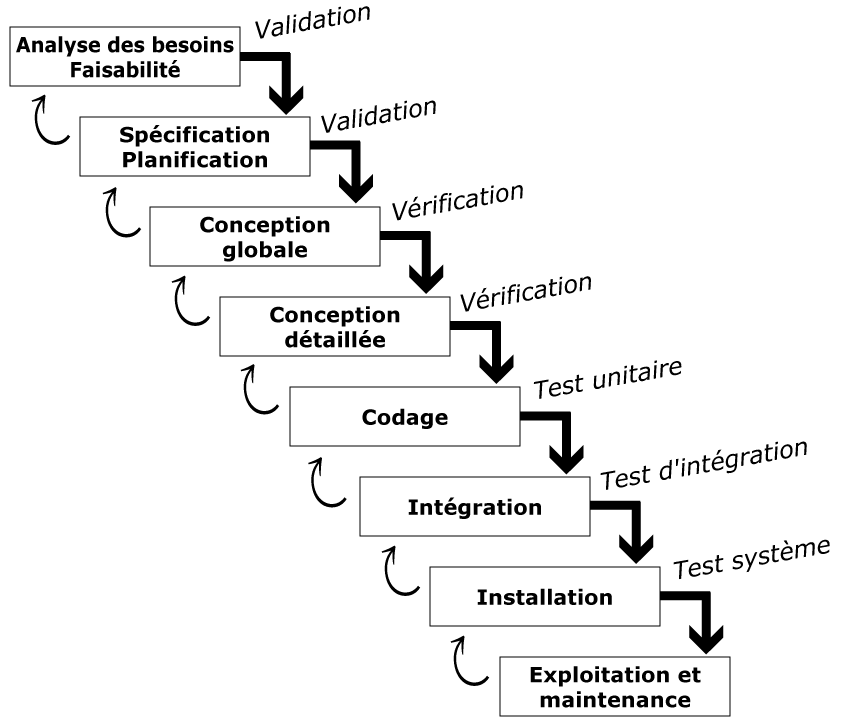
\includegraphics[width=300pt,height=300pt]{cascade.png} 
		\caption{Modèle en cascade [4]}
	\end{center}
	
\end{figure}
\clearpage
Nous avons choisi ce modèle pour sa simplicité et sa précision de tâche, ainsi qu’il ne nécessite pas une grande expérience pour développer un projet.
\subsection{Planning prévisionnel} 
Notre travail a débuté par une analyse et une conception du projet choisi. Cette phase a été suivie d’une étude théorique des outils de programmation avant d’aborder la phase de réalisation et la rédaction du rapport. 
\begin{figure}[h]
	
	\begin{center}
		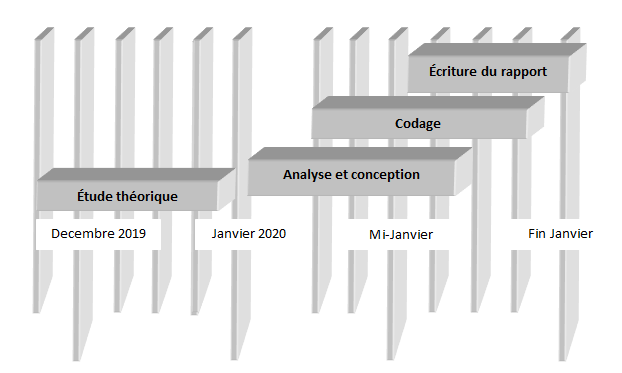
\includegraphics[width=450pt,height=400pt]{planning.png} 
		\caption{Planning}
	\end{center}
	
\end{figure}
\newpage
\begin{itemize}

\item [-] Étude théorique : L’étape de l’étude des différentes besoins, la rédaction du cahier de charges et le choix des langages et technologies du développement utilisées pour la réalisation du projet.
\item [-] Analyse et conception : L’étape de la réalisation des diagrammes et de schémas de conception utiles pour notre projet.
\item [-] Codage : L’étape de la création de la base de données et du développement de notre site web.
\end{itemize}
\section{Conclusion}
Dans ce premier chapitre, nous avons essayé de donner une vision générale sur notre projet. Nous avons défini les acteurs qui interagissent avec le site web, les besoins fonctionnels, et enfin le processus de développement suivi tout au long du projet. 

\chapter{Analyse et conception}
\newpage
\section{Introduction}

Avant de programmer le site web et se lancer dans l’écriture du code, il faut d’abord organiser les idées et les documenter, puis organiser la réalisation en définissant les modules et les étapes de la réalisation. Cette démarche s’appelle la modélisation, son produit est un module.

\section{Langage de conception }
Dans le cadre de notre projet nous avons utilisé le langage UML (Unified Modeling Language) [5] pour la modélisation des différents diagrammes.
\subsection{Présentation d’UML }
UML « Unified Modeling Language » : est un langage visuel constitué d’un ensemble des schémas, appelés diagrammes, qui donnent chacun une vision différente du projet à traiter.
UML nous fournit donc des diagrammes pour représenter le logiciel à développer : son fonctionnement, sa mise en route, les actions susceptibles d’être effectuées par le logiciel, etc.
Notre choix s'est basé sur les points forts de ce langage. UML est conçu pour s'adapter à n'importe quel langage de programmation orientée objet (POO), et présente plusieurs modèles (Diagrammes) pour une modélisation bien précise.\\

\subsection{Avantages d’UML }
\begin{itemize}
	\item [-] Universel.
	\item [-] Adopté par les grandes entreprises. 
	\item [-] Adopté par plusieurs processus de développement 
	\item [-] Limite les risques d’erreur. 
	\item [-] N’est pas limité au domaine informatique.
	
\end{itemize}
\section{Modélisation et spécification Fonctionnelles }

\subsection{Diagrammes Cas d’utilisation }
Le diagramme de cas d’utilisation a pour but de donner une vision globale sur les interfaces de la future application. C’est le premier diagramme UML constitué d’un ensemble d’acteurs qui agit sur des cas d’utilisation, le comportement d’une application du point de vue utilisateur.\\
Ci-dessous, nous présentons le diagramme de cas d’utilisation pour la compréhension du fonctionnement de l’application.\\
\begin{figure}[h]
	
	\begin{center}
		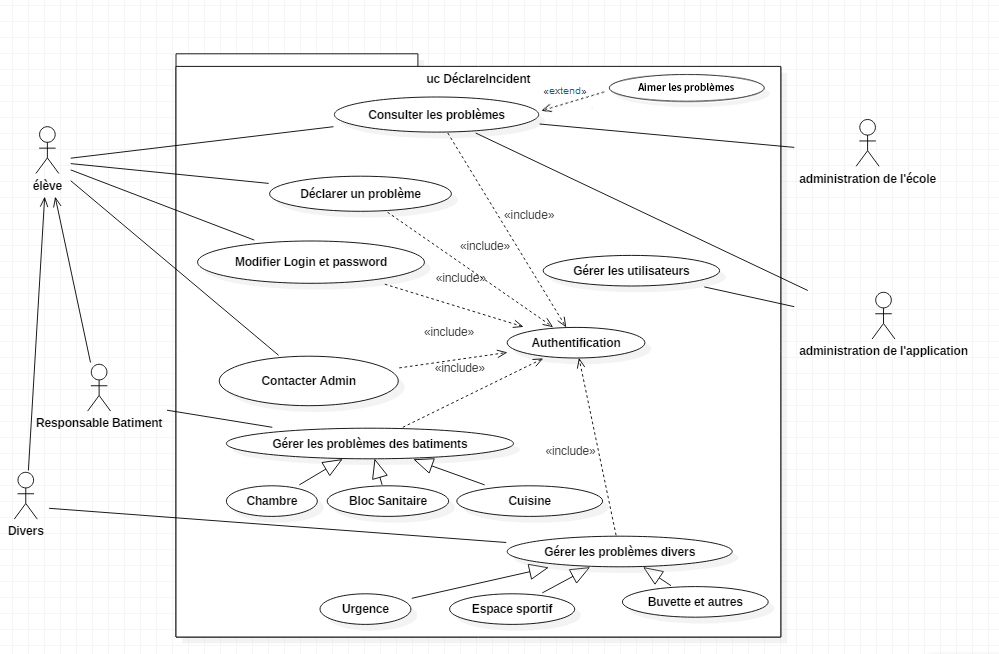
\includegraphics[width=400pt,height=400pt]{Usecase.png} 
		\caption{Diagramme de cas d'utilisation}
	\end{center}
	
\end{figure}
\newpage
\subsection{Côté élève }
Le diagramme de cas d’utilisation montre l’interaction entre l’élève et le système. On distingue donc trois services dans ce diagramme :\\
\begin{itemize}
	\item [-] Gérer le Compte.
	\item [-] Publier le problème.
	\item [-] Visualiser les problèmes.
	\item [-] Contacter les membres de comités.\\
	
\end{itemize}
Il faut que l’élève soit déjà authentifié pour profiter de ces services.

\subsubsection{Description du cas d’utilisation <Gérer le compte> }
L’élève doit initialement se connecter au site web à travers son email et son mot de passe. Puis, il clique sur le bouton profil pour voir l’ensemble des informations à remplir. Le tableau ci-dessous décrit la démarche de la gestion de compte par l’élève dans le site web.\\
\begin{table}[h]
\begin{tabular}{|l|l|}
	\hline
	\multicolumn{2}{|l|}{\bf SOMMAIRE}\\
	
	\hline
	\bf Titre : &  Gestion du profil \\
	\hline
	\bf But : & Gérer l’ensemble d’informations et la possibilité de les modifier\\
	\hline
	\bf Résumé : & L’élève clique sur profil, l’action se déclenche et un formulaire s’affiche. \\
	\hline
	\bf Acteur : & Élève \\
	\hline
	\bf Pré conditions & \bf Post conditions \\
	\hline
	 -Élève est authentifié &  \\
	\hline
	\multicolumn{2}{|l|}{\bf Scénario nominal}\\
	\hline
	 \multicolumn{2}{|l|}{\makecell[l]{1-L’élève se connecte au site web à travers son email et un mot de passe. \\2-L’élève clique sur profil et un formulaire s’affiche.}}\\
	\hline
	\multicolumn{2}{|l|}{\bf Enchainement alternatif}\\
	\hline
	\multicolumn{2}{|l|}{\makecell[l]{-L’élève n’a pas validé son choix. \\-Le site web affiche un message de confirmation.}}\\
	\hline

\end{tabular}
\caption{Description du cas d’utilisation <Gérer le profil >}
\end{table}
\newpage
\subsubsection{Description du cas d’utilisation < Publier un problème > }
L’élève doit initialement désigner son problème afin de le publier. Le tableau ci-dessous décrit la démarche de la publication du problème.\\
\begin{table}[h]
	\begin{tabular}{|l|l|}
		\hline
		\multicolumn{2}{|l|}{\bf SOMMAIRE}\\
		
		\hline
		\bf Titre : &  publier problème \\
		\hline
		\bf But : & Publication des différentes problèmes afin d’être résolus.\\
		\hline
		\bf Résumé : & \makecell[l]{L’élève clique sur « problems », l’action se déclenche et l’élève reçoit \\un formulaire  pour désigner son problème.}\\
		\hline
		\bf Acteur : & Élève \\
		\hline
		\bf Pré conditions & \bf Post conditions \\
		\hline
		-Élève est authentifié &  \\
		\hline
		\multicolumn{2}{|l|}{\bf Scénario nominal}\\
		\hline
		\multicolumn{2}{|l|}{\makecell[l]{1-L’élève clique sur <problems>. \\2-L’élève remplit le formulaire.}}\\
		\hline
		\multicolumn{2}{|l|}{\bf Enchainement alternatif}\\
		\hline
		\multicolumn{2}{|l|}{\makecell[l]{-L’élève n’a pas rempli son choix. \\-Le site web affiche un message d’erreur.}}\\
		\hline
		
	\end{tabular}
	\caption{Description du cas d’utilisation < Publier un problème >}
\end{table}
\subsection{Côté comité }
Le diagramme de cas d’utilisation montre l’interaction entre le membre de comité et le système. On distingue donc des différents services dans ce diagramme :\\
\begin{itemize}
	\item [-] Gérer le Compte.
	\item [-] Visualiser les statistiques.
	\item [-] Gérer les problèmes.
	\item [-] Visualiser l’archive.
	\item [-] Visualiser les problèmes en cours.
	\item [-] Visualiser la liste des étudiants.
	\item [-] Publier un problème.
\end{itemize}
\subsubsection{Description du cas d’utilisation <Gérer les problèmes > }
Le membre de comité doit initialement se connecter au site web à travers son email et son mot de passe. Puis, il sélectionne les problèmes à résoudre pour enfin répondre aux besoins de l’élève.\\
\begin{table}[h]
	\begin{tabular}{|l|l|}
		\hline
		\multicolumn{2}{|l|}{\bf SOMMAIRE}\\
		
		\hline
		\bf Titre : &  Gérer les problèmes \\
		\hline
	    \bf 	But : & Gestion des problèmes des étudiants.\\
		\hline
	\bf 	Résumé : & \makecell[l]{Le membre clique sur <Problems>, résout le problème et affecte un statut \\pour chaque problème.}   \\
		\hline
		\bf Acteur : & Membre de comité \\
		\hline
		\bf Pré conditions  & \bf Post conditions \\
		\hline
		-Élève est authentifié &  \\
		\hline
		\multicolumn{2}{|l|}{\bf Scénario nominal}\\
		\hline
		\multicolumn{2}{|l|}{\makecell[l]{1-Le membre se connecte au site web à travers son email et un mot de passe. \\2-Le membre sélectionne les problèmes à résoudre.\\
		3-Le membre affecte un statut pour chaque problème.}}\\
		\hline
		\multicolumn{2}{|l|}{\bf Enchainement alternatif}\\
		\hline
		\multicolumn{2}{|l|}{\makecell[l]{-Le membre n’a pas sélectionner un problème. \\-Le site web affiche un message d’erreur.}}\\
		\hline
		
	\end{tabular}
	\caption{Description du cas d’utilisation < Gérer les problèmes >}
\end{table}
\subsubsection{Description du cas d’utilisation <Visualiser statistiques> }
Le memre  doit initialement se connecter au site web à travers son email et son mot de passe. Puis, il clique sur <Statistics> et quatre boutons s’affichent. Le tableau ci-dessous décrit la démarche de la visualisation des statistiques.\\
\begin{table}[h]
	\begin{tabular}{|l|l|}
		\hline
		\multicolumn{2}{|l|}{\bf SOMMAIRE}\\
		
		\hline
		\bf Titre : &  Postuler à un emploi \\
		\hline
		\bf But : & \makecell[l]{Envoyer la candidature de recrutement au recruteur \\qui a publié l’offre.} \\
		\hline
		\bf Résumé : & \makecell[l]{Le candidat clique sur le bouton postuler et sa\\candidature est envoyée directement au recruteur.}   \\
		\hline
		\bf Acteur : & Candidat \\
		\hline
		\bf Pré conditions & \bf Post conditions \\
		\hline
		\makecell[l]{-Le candidat est authentifié \\-L’emploi doit être déjà publié par un recruteur.}
		 &  \\
		\hline
		\multicolumn{2}{|l|}{\bf Scénario nominal}\\
		\hline
		\multicolumn{2}{|l|}{\makecell[l]{1-Le candidat se connecte  à travers son email et un mot de passe. \\2-Le candidat choisit l’offre convenable.\\
				3-Le candidat clique sur le bouton postuler et sa candidature  est envoyée au recruteur.}}\\
		\hline
		\multicolumn{2}{|l|}{\bf Enchainement alternatif}\\
		\hline
		\multicolumn{2}{|l|}{\makecell[l]{-L’offre d’emploi n’existe plus. \\-Le site web  affiche un message d’erreur.}}\\
		\hline
		
	\end{tabular}
	\caption{Description du cas d’utilisation <Postuler un emploi>}
\end{table}
\newpage
\section{Conception}
\subsubsection{Diagrammes de séquence}
Les diagrammes de séquence peuvent servir à illustrer les cas d’utilisations décrits précédemment. Ils permettent de représenter la succession chronologique des opérations réalisées par un acteur et qui font passer d’un objet à un autre pour représenter un scénario.
Initialement, l’utilisateur s’inscrit  en tant que recruteur pour bénéficier des différents services disponibles dans le site web.\\
\begin{figure}[h]
	
	\begin{center}
		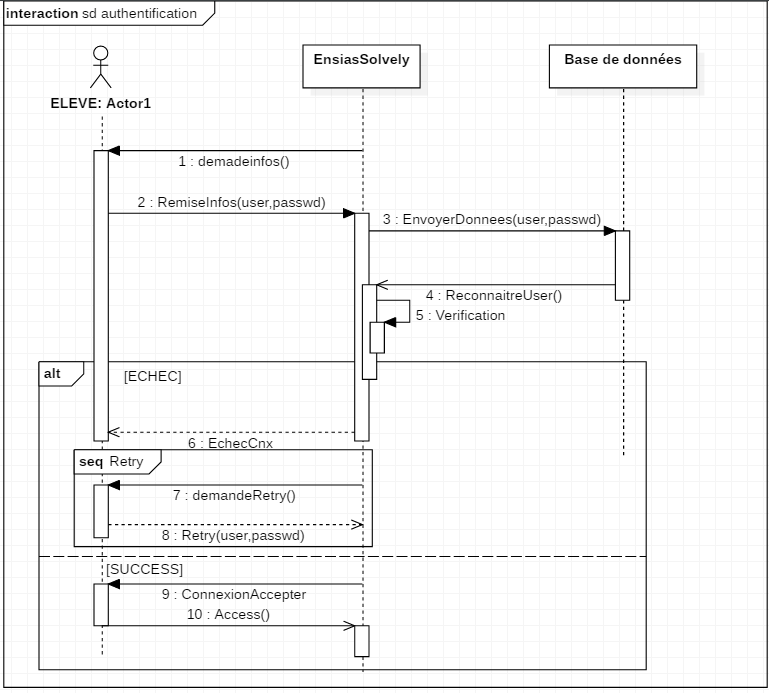
\includegraphics[width=400pt,height=400pt]{seq1.png} 
		\caption{Diagramme de séquence d'authentification}
	\end{center}
	
\end{figure}
\newpage
L’élève peut ainsi déclarer le problème rencontré la situation se résume comme suit.\\

\begin{figure}[h]
	
	\begin{center}
		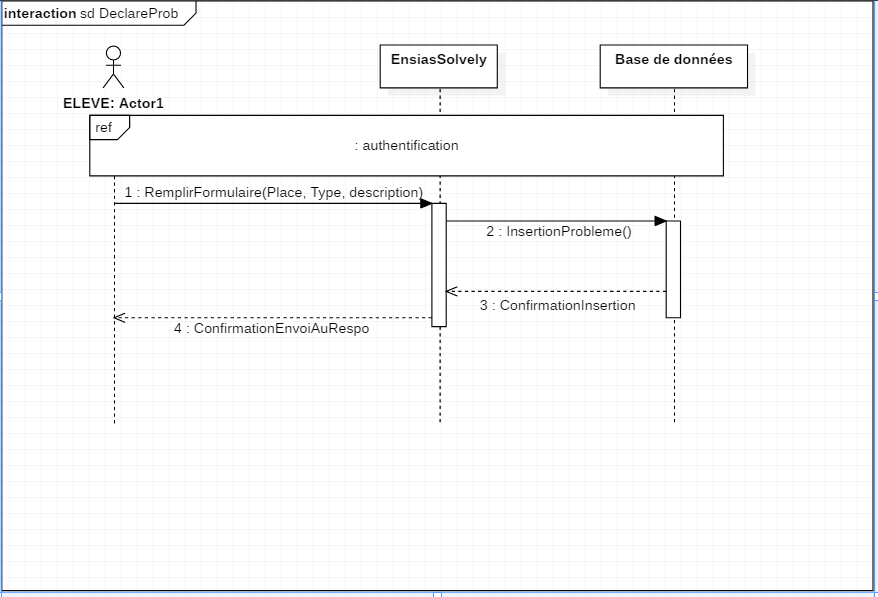
\includegraphics[width=400pt,height=400pt]{seq2.png} 
		\caption{Diagramme de séquence de déclaration de problème}
	\end{center}
	
\end{figure}
\newpage
Le membre de comité doit régler dans les plus brefs délais le problème rencontré par l’étudiant.\\
\begin{figure}[h]
	
	\begin{center}
		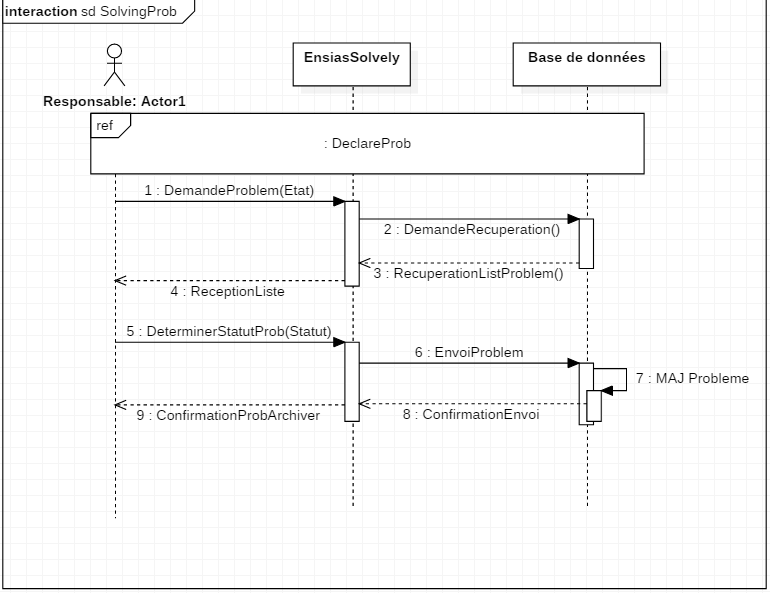
\includegraphics[width=400pt,height=400pt]{seq3.png} 
		\caption{Diagramme de séquence de résolution de problème}
	\end{center}
	
\end{figure}
\newpage
Puis, l’élève peut visualiser son archive.\\
\begin{figure}[h]
	
	\begin{center}
		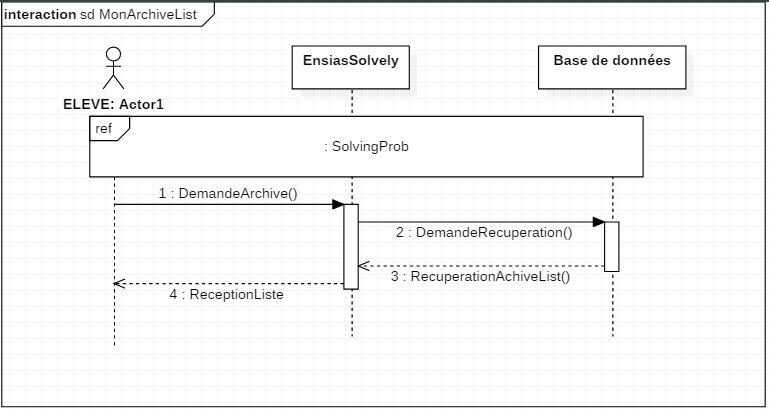
\includegraphics[width=400pt,height=400pt]{seq4.png} 
		\caption{Diagramme de séquence de visualisation d'archive de l'élève}
	\end{center}
	
\end{figure}
\newpage
L’élève peut visualiser clairement son profil, ainsi qu’il a la possibilité de modifier quelques informations.\\
\begin{figure}[h]
	
	\begin{center}
		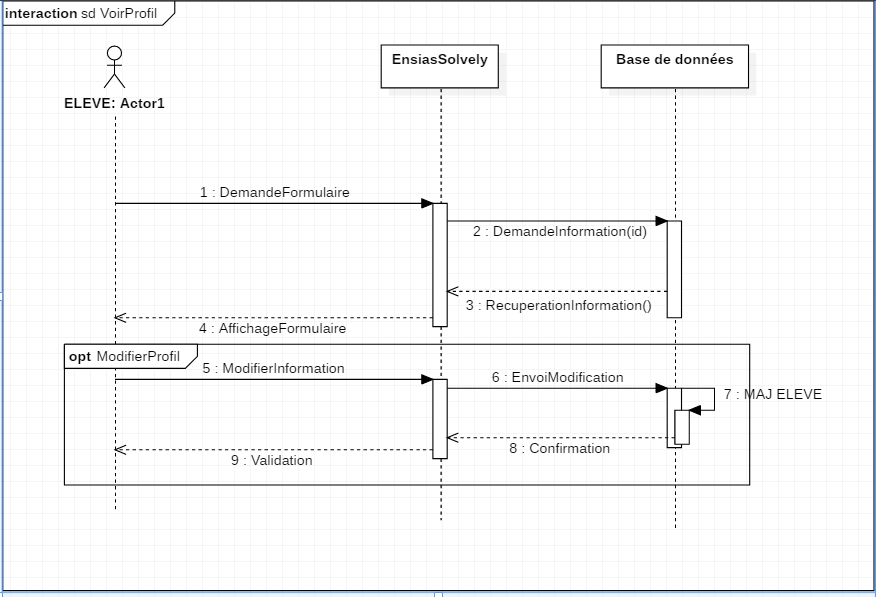
\includegraphics[width=400pt,height=400pt]{seq5.png} 
		\caption{Diagramme de séquence de visualisation de profil}
	\end{center}
	
\end{figure}
\newpage
Le membre de comité peut ainsi voir l’archive de l’ensemble des étudiants .\\
\begin{figure}[h]
	
	\begin{center}
		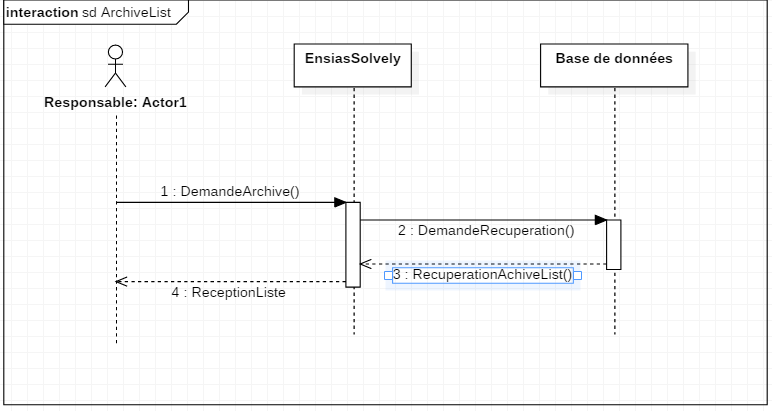
\includegraphics[width=400pt,height=400pt]{seq6.png} 
		\caption{Diagramme de séquence de visualisation de l'archive de tous les étudiants}
	\end{center}
	
\end{figure}
\newpage
Le membre de comité peut ainsi visualiser la liste des différents étudiant.\\
\begin{figure}[h]
	
	\begin{center}
		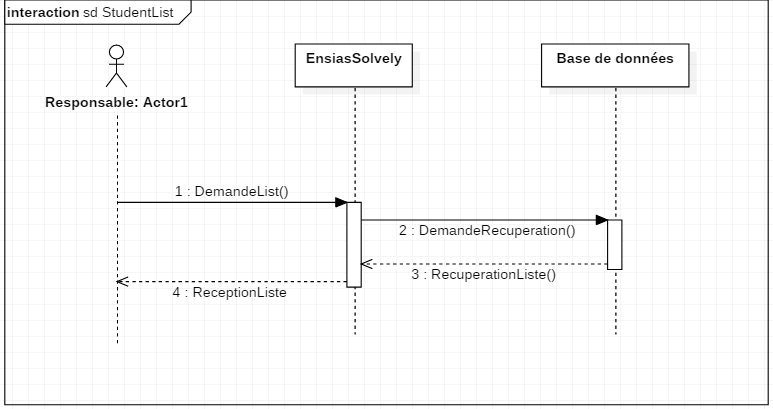
\includegraphics[width=400pt,height=400pt]{seq7.png} 
		\caption{Diagramme de séquence de visualisation de la liste des étudiants}
	\end{center}
	
\end{figure}
\newpage
\subsubsection{Diagramme d’états-transition}
L’élève peut passer par des différents statuts lors de son existence à l’école, cela se résume dans le diagramme suivant :\\
\begin{figure}[h]
	
	\begin{center}
		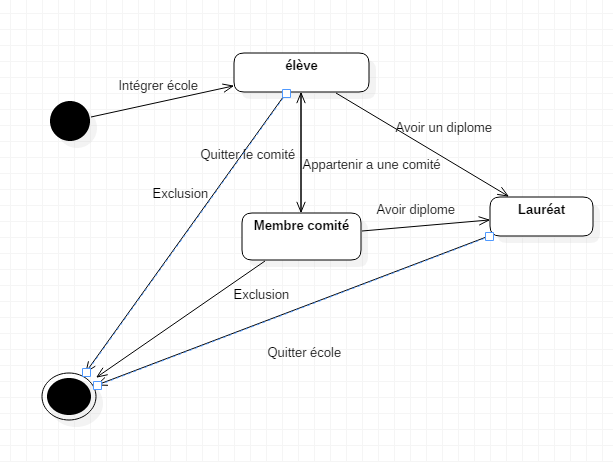
\includegraphics[width=400pt,height=400pt]{etat_trans.png} 
		\caption{Diagramme d'états transitions}
	\end{center}
	
\end{figure}
\newpage
\chapter{Création de la base de données}
\newpage
\section{Introduction}
Dans ce chapitre, nous allons décrire les étapes de création de la base de données.\\
\section{Diagramme de classe}
Le traitement de la base de données représente un grand défi pour la plupart des site-web, c’est pour cela que nous avons pris beaucoup de temps afin d’optimiser notre travail et d’extraire les tables nécessaires. Pour cela, nous avons établis le diagramme de classe afin de faciliter notre travail.\\
\begin{figure}[h]
	
	\begin{center}
		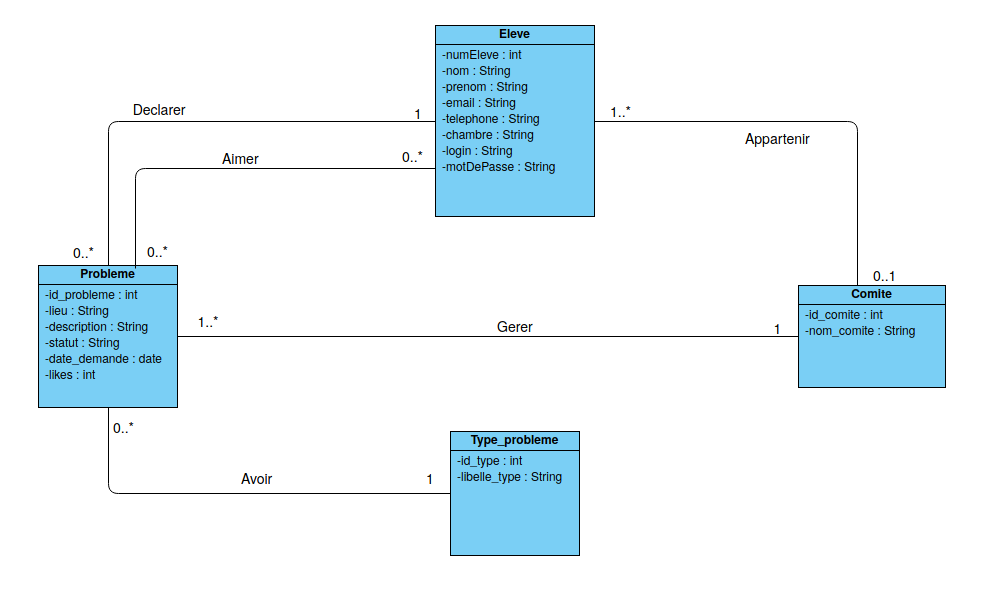
\includegraphics[width=400pt,height=400pt]{class.png} 
		\caption{Diagramme de classe}
	\end{center}
	
\end{figure}
\section{Tables de la base de données}
\subsubsection{\underline{eleve}}
\begin{table}[h]
	\begin{center}
	
	
	\begin{tabular}{|l|l|l|l|l|}
		\hline
		\begin{bf}Colonne\end{bf} & \begin{bf}Type\end{bf} & \begin{bf}Null\end{bf} & \begin{bf}Valeur par défaut\end{bf} & \begin{bf}Commentaire\end{bf}  \\
		\hline
		numEleve(primaire) & int(11) & Non & & \\
		\hline
		nom & varchar(50) & Oui &Null & \\
		\hline
		prenom & varchar(50) &Oui &Null & \\
		\hline
		email & varchar(50) & Oui &Null & \\
		\hline
		telephone & varchar(50) & Oui &Null & \\
		\hline
		chambre & varchar(50) &Oui &Null & \\
		\hline
		login & varchar(50) & Oui &Null & \\
		\hline
		motDePasse & varchar(100) & Oui &Null & \\
		\hline
		id\_comite & int(11) & Oui &Null & \\
		\hline
		
		
		
	\end{tabular}
	\caption{Table eleve}
\end{center}
\end{table}
\subsubsection{\underline{probleme}}
\begin{table}[h]
	\begin{center}
	
	\begin{tabular}{|l|l|l|l|l|}
		\hline
		\begin{bf}Colonne\end{bf} & \begin{bf}Type\end{bf} & \begin{bf}Null\end{bf} & \begin{bf}Valeur par défaut\end{bf} & \begin{bf}Commentaire\end{bf}  \\
		\hline
		id\_probleme(primaire) & int(11) & Non & & \\
		\hline
		lieu & varchar(100) & Oui &Null & \\
		\hline
		description & varchar(300) & Oui &Null & \\
		\hline
		date\_demande & date & Oui &Null & \\
		\hline
		statut & varchar(50) & Oui &Null & \\
		\hline
		id\_comite & int(11) & Non & & \\
		\hline
		login & varchar(50) & Non & & \\
		\hline
		motDePasse & varchar(100) & Non & & \\
		\hline
		numEleve & int(11) & Non & & \\
		\hline
		id\_type & int(11) & Non & & \\
		\hline
		likes & int(11) & Non &0 & \\
		\hline
		
		
		
	\end{tabular}
	\caption{Table probleme}
\end{center}
\end{table}
\subsubsection{\underline{comite}}
\begin{table}[h]
	\begin{center}
	\begin{tabular}{|l|l|l|l|l|}
		\hline
		\begin{bf}Colonne\end{bf} & \begin{bf}Type\end{bf} & \begin{bf}Null\end{bf} & \begin{bf}Valeur par défaut\end{bf} & \begin{bf}Commentaire\end{bf}  \\
		\hline
		id\_comite(primaire) & int(11) & Non & & \\
		\hline
		nom\_comite & varchar(100) & Oui &Null & \\
		\hline
		
		
	\end{tabular}
	\caption{Table comite}
\end{center}
\end{table}
\newpage
\subsubsection{\underline{boite}}
\begin{table}[h]
	\begin{center}
	\begin{tabular}{|l|l|l|l|l|}
		\hline
		\begin{bf}Colonne\end{bf} & \begin{bf}Type\end{bf} & \begin{bf}Null\end{bf} & \begin{bf}Valeur par défaut\end{bf} & \begin{bf}Commentaire\end{bf}  \\
		\hline
		numboite(primaire) & int(11) & Non & & \\
		\hline
		message & varchar(300) & Oui &Null & \\
		\hline
		numEleve & int(11) & Oui &Null & \\
		\hline
		
		
	\end{tabular}
	\caption{Table boite}
\end{center}
\end{table}
\subsubsection{\underline{aimer}}
\begin{table}[h]
	\begin{center}
	\begin{tabular}{|l|l|l|l|l|}
		\hline
		\begin{bf}Colonne\end{bf} & \begin{bf}Type\end{bf} & \begin{bf}Null\end{bf} & \begin{bf}Valeur par défaut\end{bf} & \begin{bf}Commentaire\end{bf}  \\
		\hline
		id\_probleme & int(11) & Non & & \\
		\hline
		numEleve & int(11) & Non & & \\
		\hline
		
		
	\end{tabular}
	\caption{Table aimer}
\end{center}
\end{table}
\section{Conclusion }
La bonne gestion de la base de données est le plus grand défi que rencontre chaque programmeur, c’est pour cela qu’il faut la manipuler avec prudence afin de bien gérer la totalité du travail et pour passer à la partie de la réalisation d’un site web dynamique.
\chapter{Réalisation}
\newpage
\section{Introduction}
Cette partie constitue le dernier volet de ce rapport. Après avoir terminé la phase de spécification et conception, nous présentons l’environnement matériel et logiciel utilisés pour le développement de notre site web.\\
\section{Environnement Logiciel }
\begin{itemize}
	\item [-] Eclipse : Eclipse est l’Environnement de Développement Intégré (ou IDE) le plus largement utilisé pour la programmation Java, très performant, il est de plus gratuit et open source.
	\item [-] WampServer : WampServer est une plate-forme de développement Web sous Windows pour des applications Web dynamiques à l’aide du serveur Apache2, du langage de scripts PHP et d’une base de données MySQL. Il possède également PHPMyAdmin pour gérer plus facilement les bases de données.
	\item [-] StarUML : C’est un logiciel de modélisation UML utilisé dans la conception de diagrammes et de figures.
	\item [-] Apache Tomcat : C’est un conteneur web libre de servlets et JSP Java EE. Issu du projet Jakarta, c'est un des nombreux projets de l’Apache Software Foundation. Il implémente les spécifications des servlets et des JSP, est paramétrable par des fichiers XML et des propriétés, et inclut des outils pour la configuration et la gestion. Il comporte également un serveur HTTP.
	\item [-] Jasper report : JasperReports est un outil de reporting open source, offert sous forme d'une bibliothèque qui peut être embarquée dans tous types d'applications Java.
\end{itemize}
\section{Technologies utilisées }
\begin{itemize}
	\item [-] JAVA : Java est un langage de programmation orienté objet, développé par Sun Microsystems et destiné à fonctionner dans une machine virtuelle, il permet de créer des logiciels compatibles avec des nombreux systèmes d’exploitation.
	\item [-] XML : C’est un langage nécessaire pour développer une application Android. XML n’est pas un langage de programmation mais c’est un langage informatique de balisage générique. Il sert essentiellement à stocker/transférer des données de type texte Unicode structurées en champs arborescents.
	\item [-] JEE : Cette plate-forme J2EE est une suite robuste de services middleware qui simplifie la tâche des développeurs d’applications côté serveur. Elle repose sur les technologies existantes de la plate-forme J2SE afin de faciliter la création d’applications.

\end{itemize}
\section{Architecture de l’application }
\subsection{Client / Serveur }
\begin{figure}[h]
	
	\begin{center}
		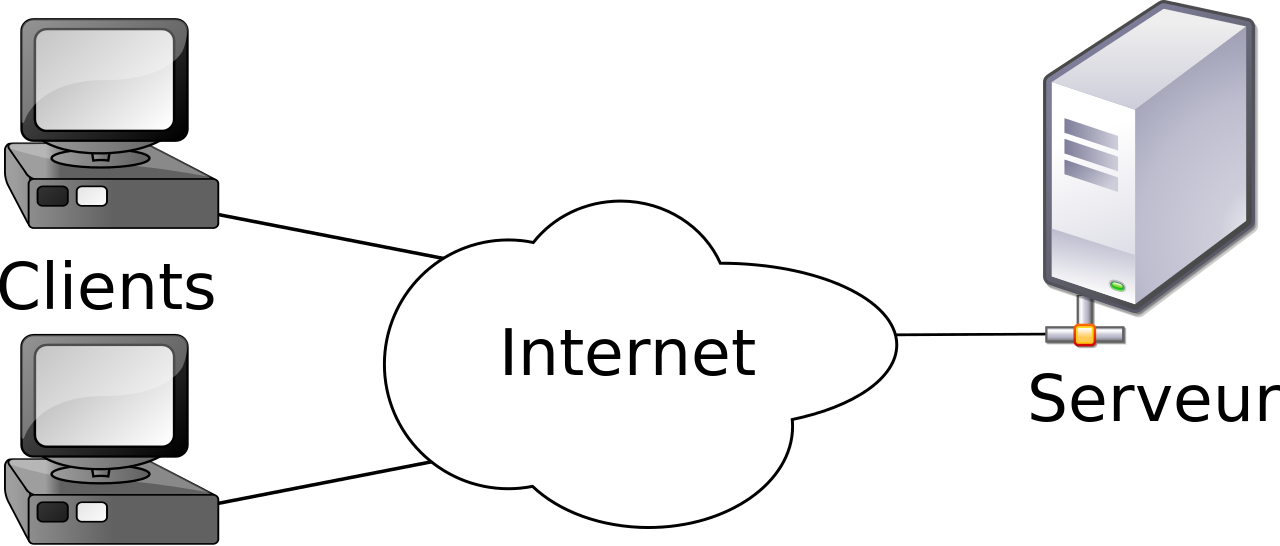
\includegraphics[width=300pt,height=300pt]{clientserveur.png} 
		\caption{Connexion Clients/Serveur [7]}
	\end{center}
	
\end{figure}
\newpage
Dans l’architecture à trois niveaux, les applications au niveau serveur sont délocalisées, c’est- à-dire que chaque serveur est spécialisé dans une tâche (serveur web/ serveur de base de données par exemple).
Il permet :\\
\begin{itemize}
	\item [-] Une plus grande flexibilité et souplesse. 
	\item [-] Une sécurité accrue car la sécurité peur être définie indépendamment pour chaque service, et à chaque niveau. 
	\item [-] Une meilleure performance, étant donné le partage des tâches entre les différents serveurs.\\
\end{itemize}
Protocole de communication :\\
Dans notre projet, nous avons utilisé le protocole HTTP, afin de communiquer les données entre la partie client et le serveur web. Le HTTP est un protocole qui définit la communication entre un serveur et un client. Nous utilisons la méthode Post pour envoyer des données au programme situé à une URL spécifiée.
\subsection{Architecture MVC }
Le modèle MVC décrit une manière d’architecturer une application informatique en la décomposant en trois sous-parties :\\
\begin{itemize}
	\item [-] La partie Modèle.
	\item [-] La partie Vue.
	\item [-] La partie Contrôleur.
\end{itemize}
Voici à la figure suivante le schéma représentant l’architecture MVC : \\
\begin{figure}[h]
	
	\begin{center}
		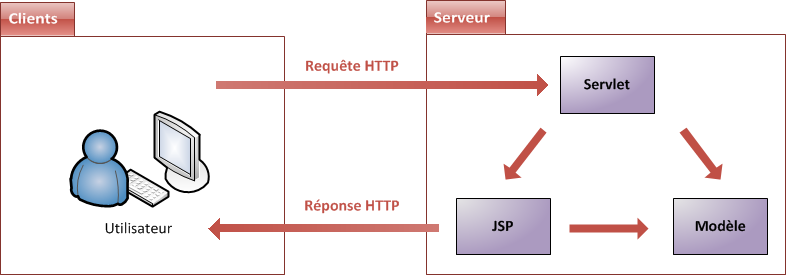
\includegraphics[width=300pt,height=150pt]{mvc.png} 
		\caption{Architecture MVC [7]}
	\end{center}
	
\end{figure}
\newpage
Nous avons donc codé notre site en mettant en place ce modèle :\\
\begin{itemize}
	\item [-] création des beans qui enregistrent les données saisies et validées.
	\item [-] création des objets comportant les méthodes de récupération/conversion/validation des contenus des champs des formulaires du site web.
	\item [-] les servlets n'interviennent plus directement sur les données des requêtes, mais aiguillent simplement les requêtes entrantes. 
	\item [-] Les JSP sont adaptées au modèle MVC.
\end{itemize}
\section{Interfaces de l'application}
Dans cette partie on décrit les différents interfaces de notre application web.\\
La page d'accueille est comme suit:\\
\begin{figure}[h]
	
	\begin{center}
		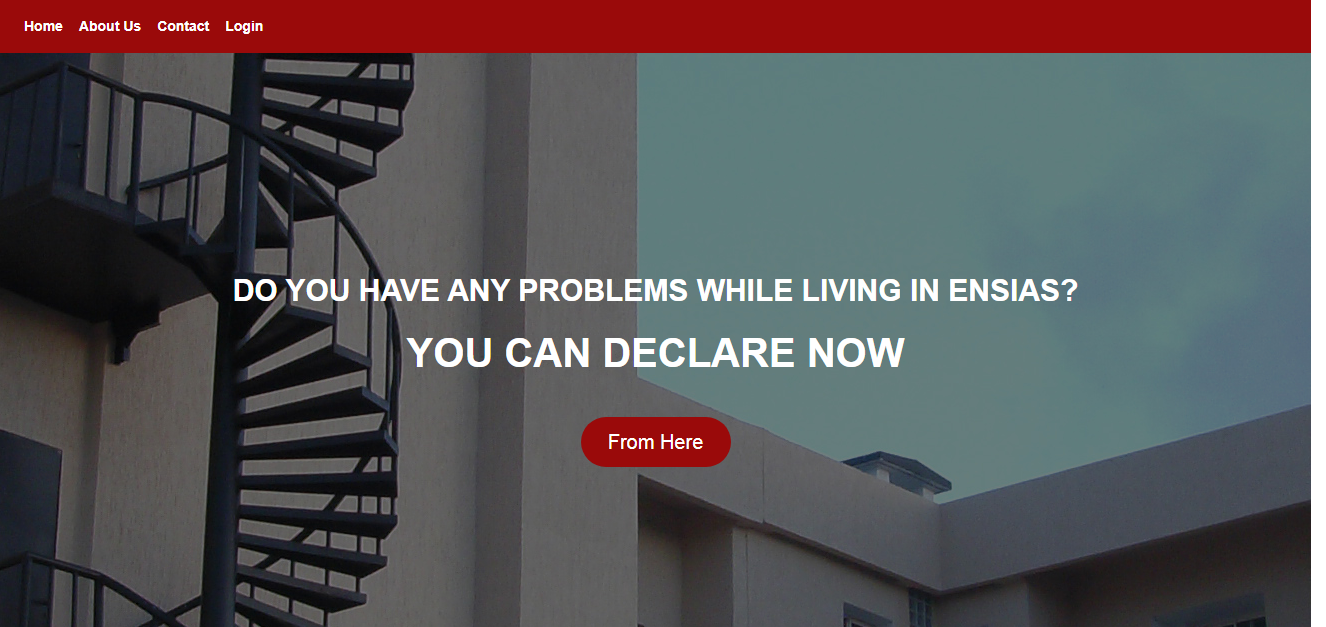
\includegraphics[width=500pt,height=300pt]{home.png} 
		\caption{Page d'accueil}
	\end{center}
	
\end{figure}
\newpage
L'utilisateur peut donc se connecter en cliquant sur 'Login' ou bien 'From Here'.\\
\begin{figure}[h]
	
	\begin{center}
		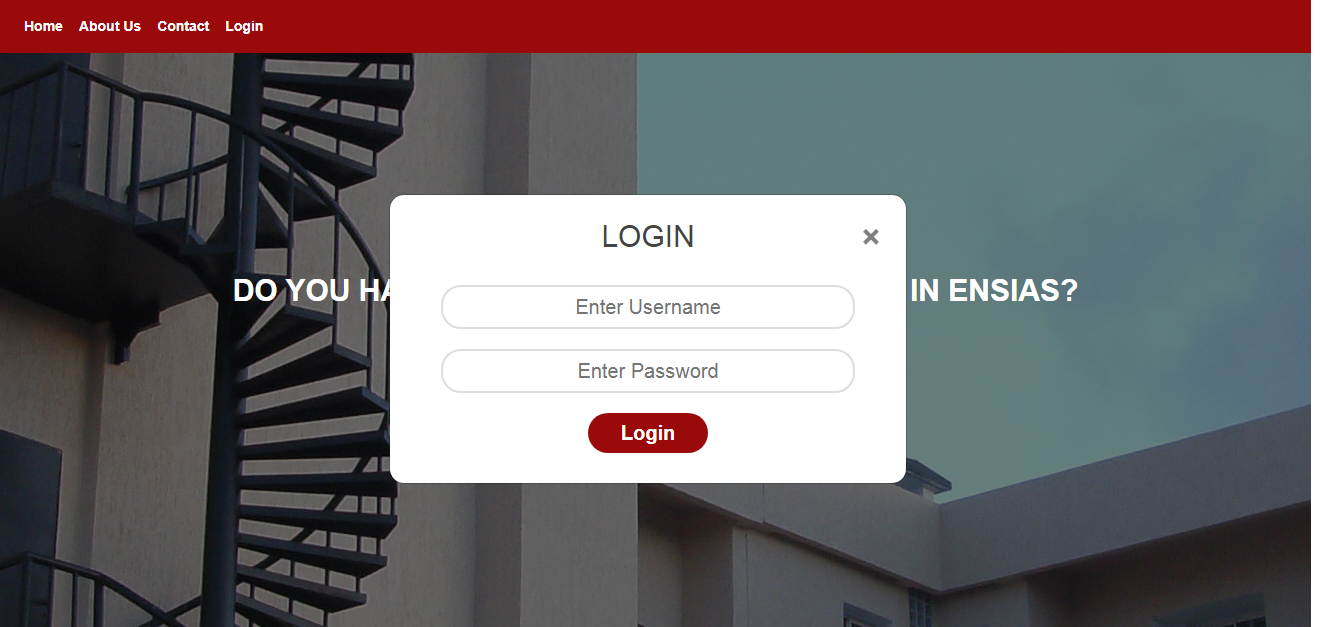
\includegraphics[width=500pt,height=300pt]{login.png} 
		\caption{Fenêtre de login}
	\end{center}
	
\end{figure}
\newpage
Si l'utilisateur est membre d'une comité, alors il se connecte en mode admin .\\
\begin{figure}[h]
	
	\begin{center}
		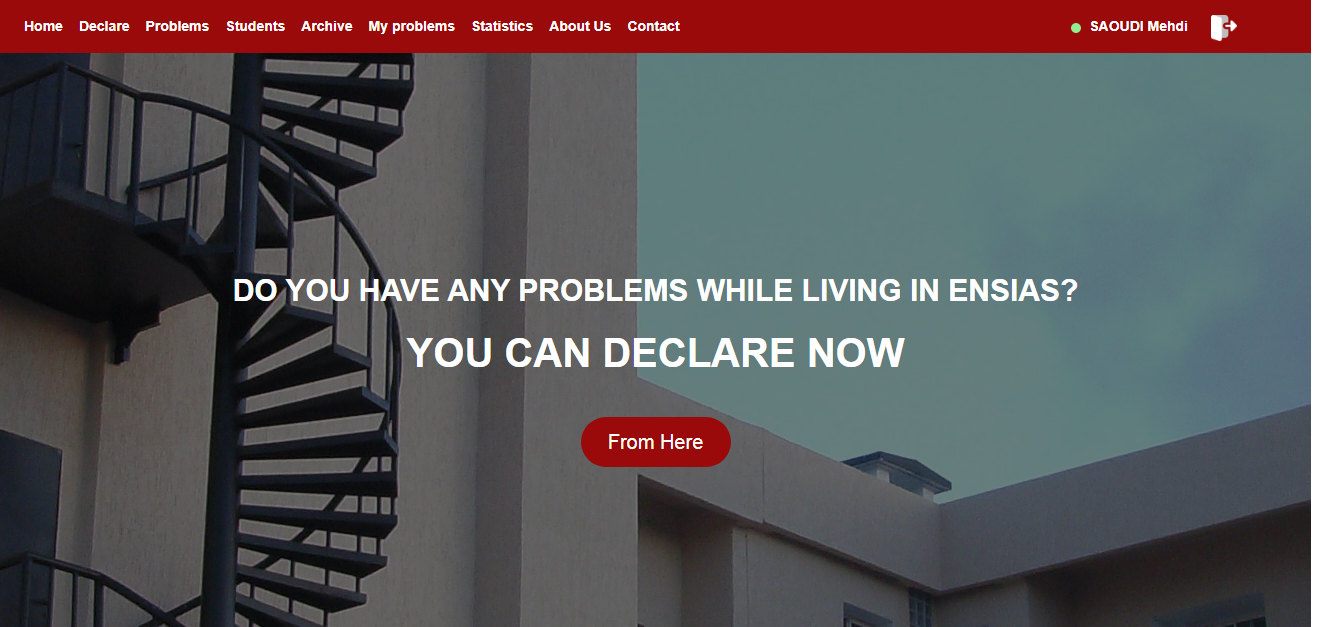
\includegraphics[width=500pt,height=300pt]{home-admin.png} 
		\caption{Interface de l'admin}
	\end{center}
	
\end{figure}
\newpage

Un élève peut déclarer un problème en cliquant sur 'Declare' ou bien 'From Here'.\\
\begin{figure}[h]
	
	\begin{center}
		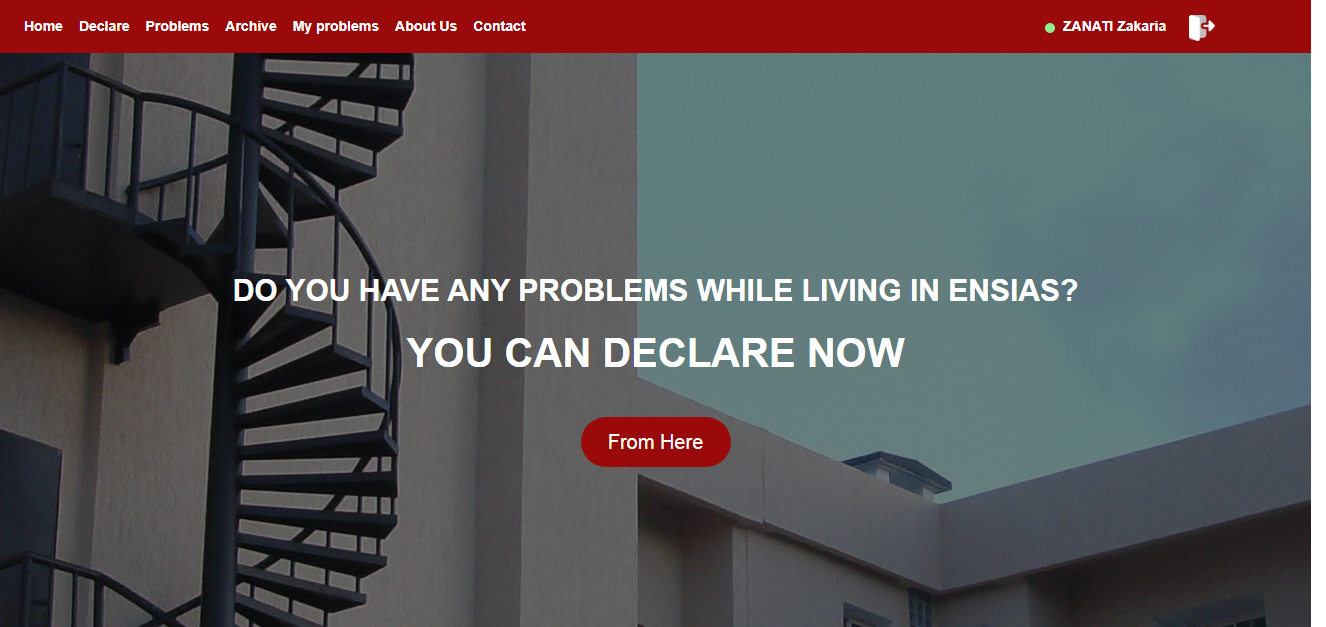
\includegraphics[width=500pt,height=300pt]{home-eleve.png} 
		\caption{Interface de l'élève}
	\end{center}
	
\end{figure}
\newpage
Il saisit en suite les détail de son problème puis il l'envoie.\\
\begin{figure}[h]
	
	\begin{center}
		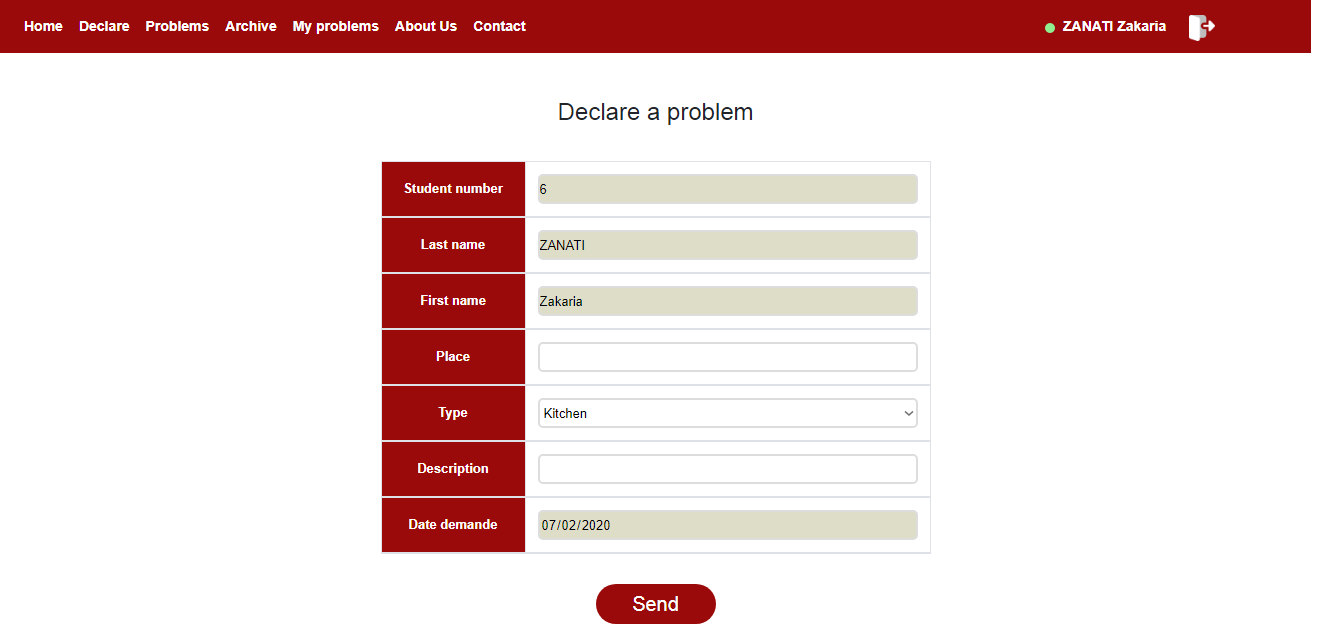
\includegraphics[width=500pt,height=300pt]{declare.png} 
		\caption{Page de déclaration de problèmes}
	\end{center}
	
\end{figure}
\newpage
Tous les élèves ont le droit de consulter la liste de tous les problèmes déclaré.
Un élève peut cliquer sur 'j'aime' s'il a le même problème qu'un autre élève qui l'a déjà déclaré, plus un problème a des "j'aime" plus il monte en haut et devient plus prioritaire. Avec cette fonction on évitera d'avoir plusieurs problèmes avec la même description.\\
\begin{figure}[h]
	
	\begin{center}
		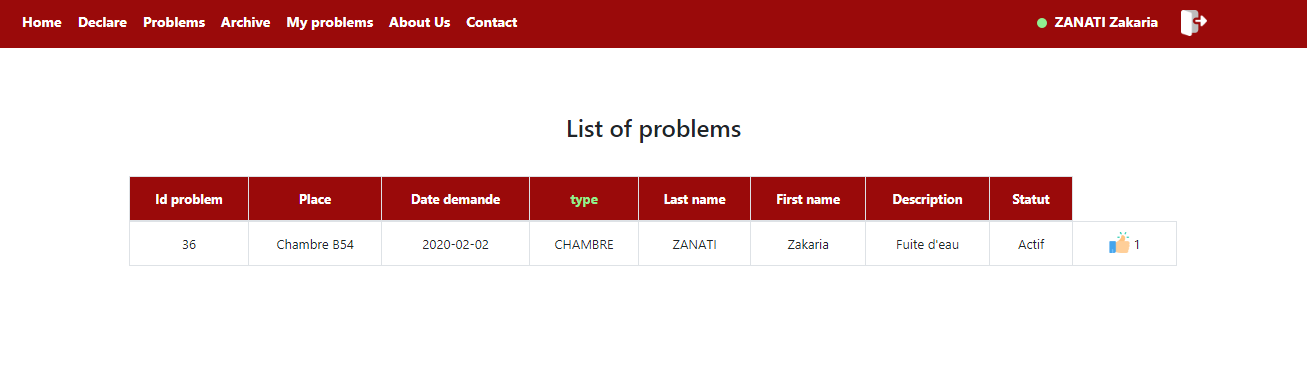
\includegraphics[width=500pt,height=300pt]{problems-eleve.png} 
		\caption{Liste des problèmes de tous les élèves}
	\end{center}
	
\end{figure}
\newpage
\begin{figure}[h]
	
	\begin{center}
		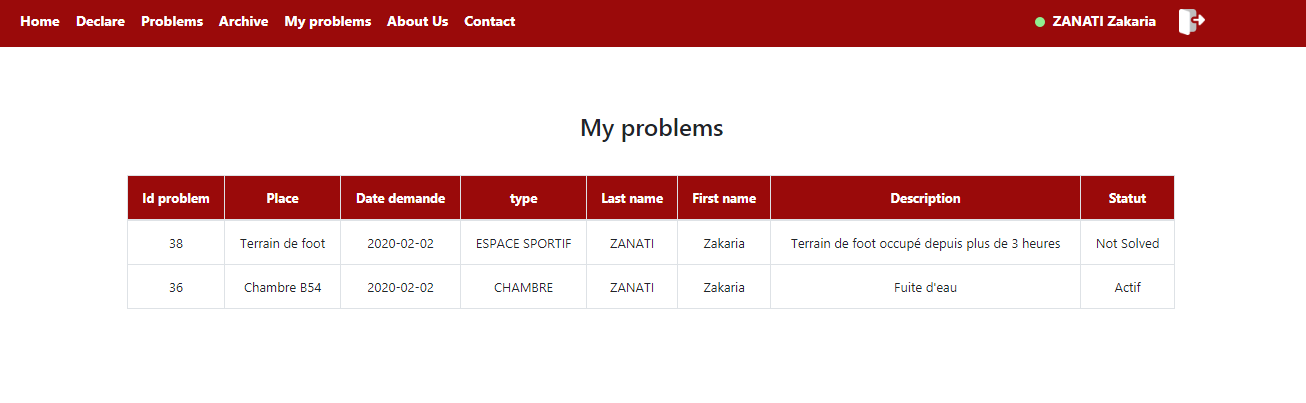
\includegraphics[width=500pt,height=300pt]{myproblems.png} 
		\caption{Liste des problèmes d'un élève}
	\end{center}
	
\end{figure}
\newpage
Chaque élève a le droit de modifier ses informations personnelles.\\
\begin{figure}[h]
	
	\begin{center}
		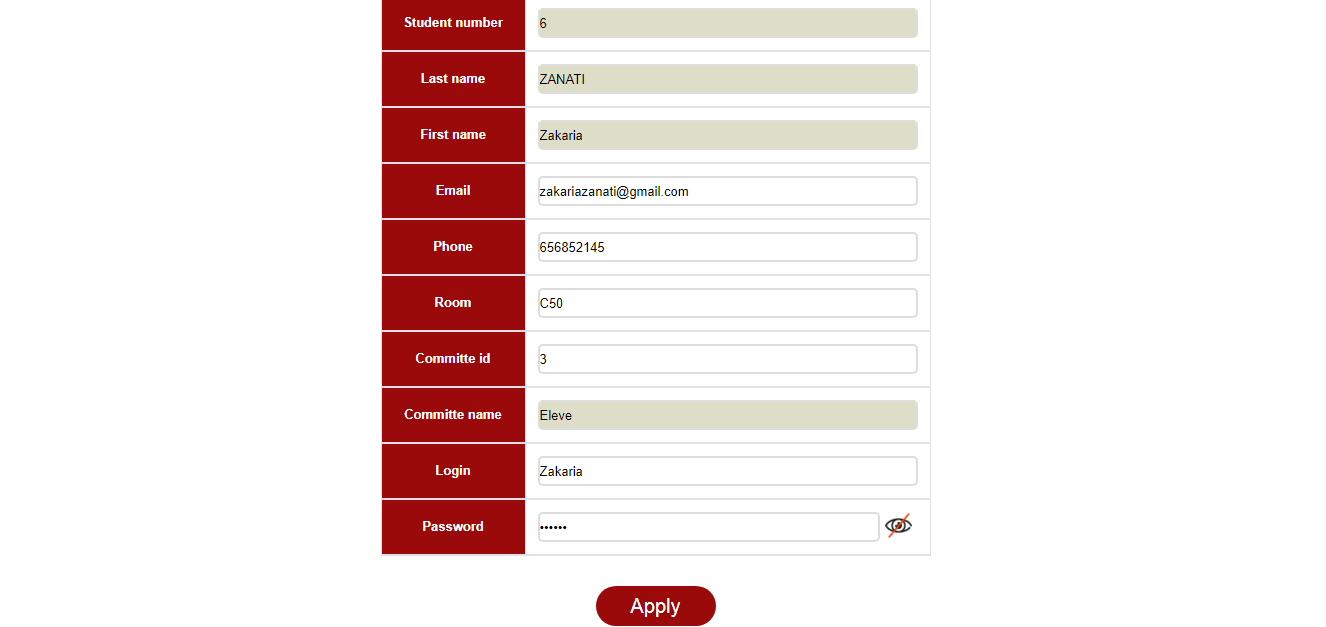
\includegraphics[width=500pt,height=300pt]{profile.png} 
		\caption{Profil de l'élève}
	\end{center}
	
\end{figure}
\newpage
Un admin peut changer l'état d'un problème en 'solved' ou bien 'not solved'.
\begin{figure}[h]
	
	\begin{center}
		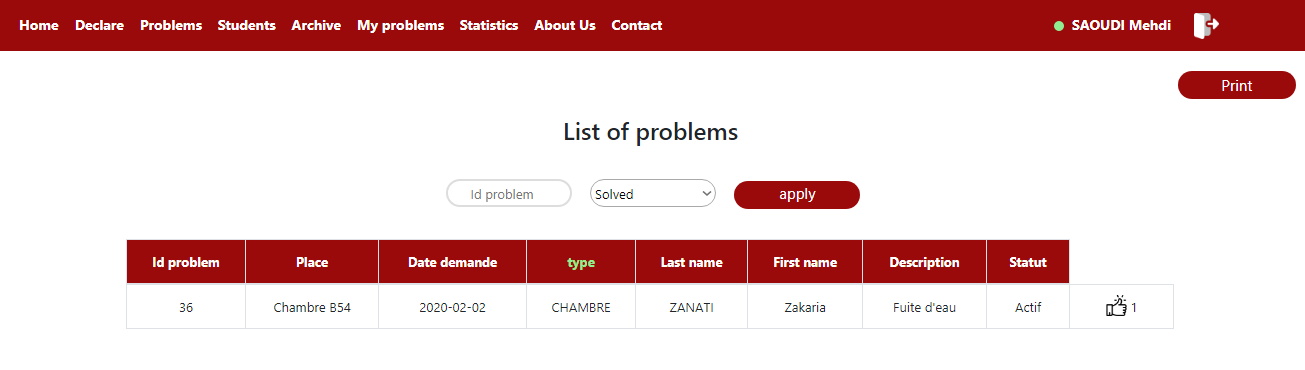
\includegraphics[width=500pt,height=300pt]{problems-admin.png} 
		\caption{Liste de tous les problèmes }
	\end{center}
	
\end{figure}
\newpage
Il peut consulter les problèmes urgent en cliquant sur 'type'.\\
\begin{figure}[h]
	
	\begin{center}
		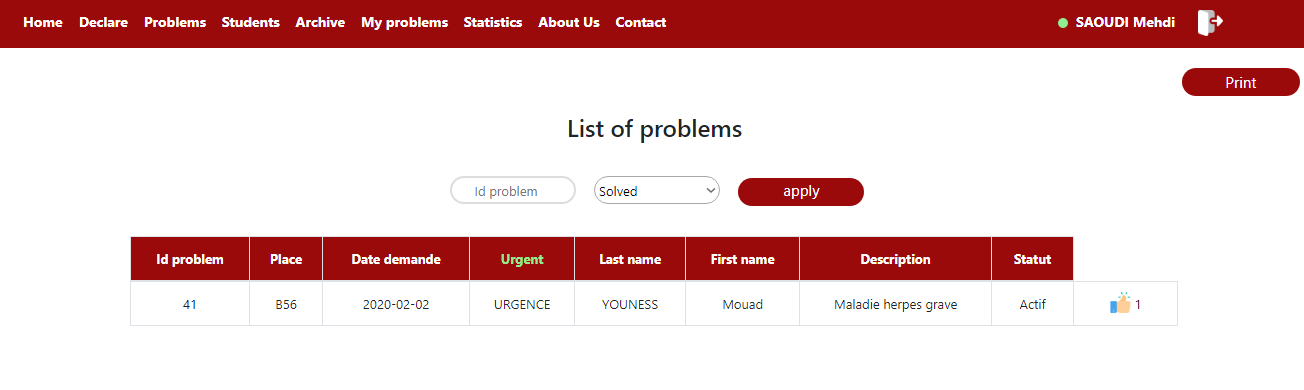
\includegraphics[width=500pt,height=300pt]{urgence.png} 
		\caption{Liste des problèmes urgent}
	\end{center}
	
\end{figure}
\newpage
Il peut aussi consulter l'archive de tous les problèmes déjà déclaré.\\
\begin{figure}[h]
	
	\begin{center}
		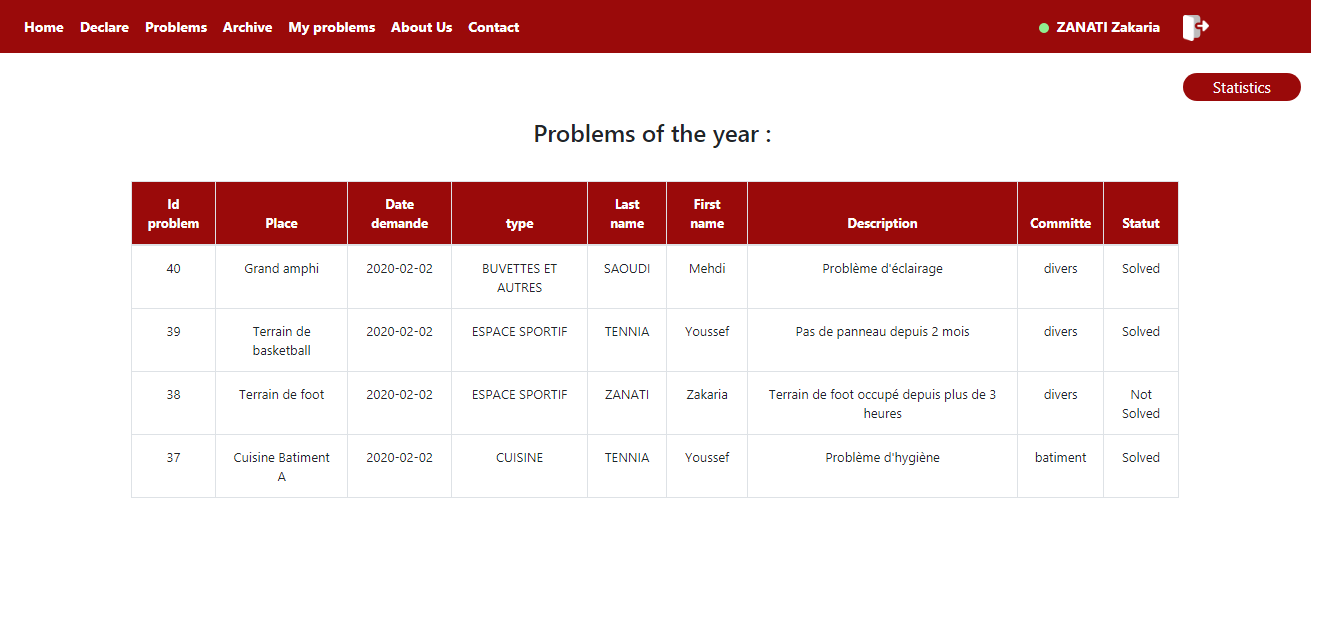
\includegraphics[width=500pt,height=300pt]{archive.png} 
		\caption{Page d'archive}
	\end{center}
	
\end{figure}
\newpage
Il peut récupérer la liste des problèmes et la liste globale des étudiants.\\
\begin{figure}[h]
	
	\begin{center}
		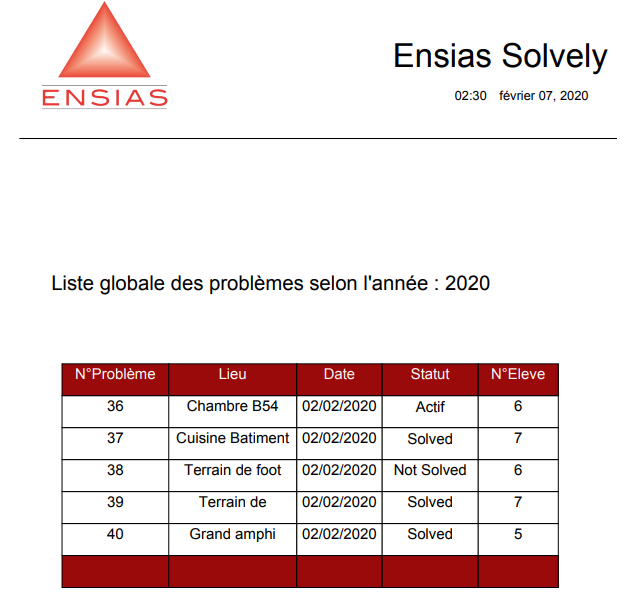
\includegraphics[width=500pt,height=400pt]{listproblems.png} 
		\caption{Liste des problèmes de l'année en cours}
	\end{center}
	
\end{figure}
\newpage
\begin{figure}[h]
	
	\begin{center}
		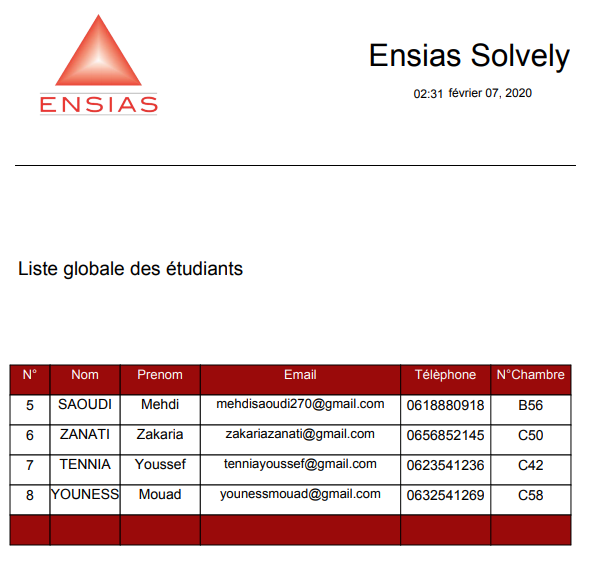
\includegraphics[width=500pt,height=400pt]{studentslist.png} 
		\caption{Liste des étudiants}
	\end{center}
	
\end{figure}
\newpage
Chaque étudiant a un code qr généré automatiquement par l'application web pour s'authentifier.\\
\begin{figure}[h]
	
	\begin{center}
		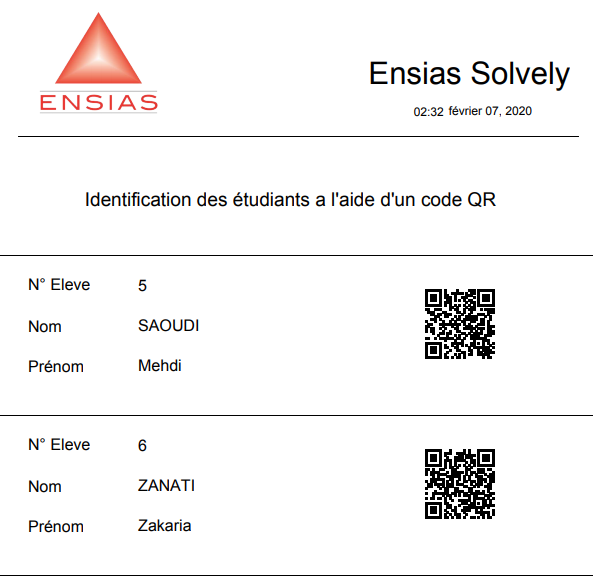
\includegraphics[width=500pt,height=400pt]{studentsqr.png} 
		\caption{Qr code des étudiants}
	\end{center}
	
\end{figure}
\newpage
Quelques statistiques sur la distribution et la résolution des problèmes.\\ 
\begin{figure}[h]
	
	\begin{center}
		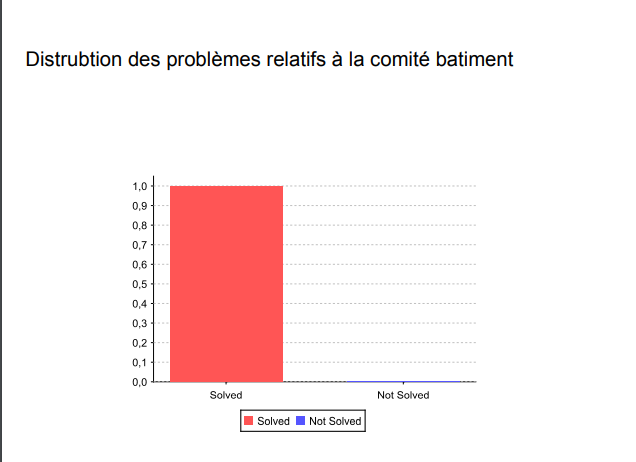
\includegraphics[width=500pt,height=400pt]{d1.png} 
		\caption{Distribution des problèmes de la comité bâtiments}
	\end{center}
	
\end{figure}

\newpage
\begin{figure}[h]
	
	\begin{center}
		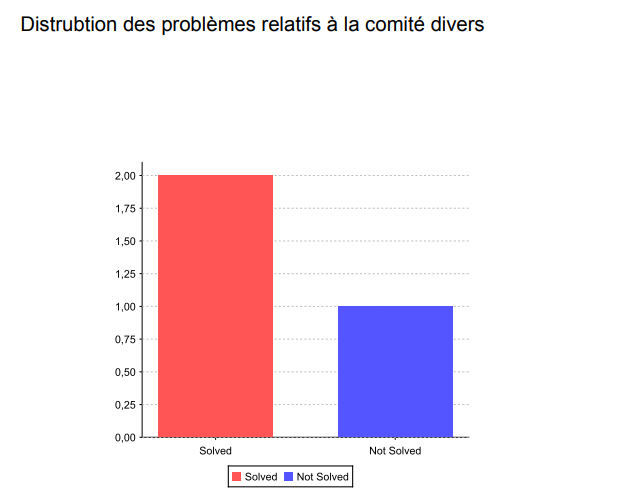
\includegraphics[width=500pt,height=400pt]{d3.png} 
		\caption{Distribution des problèmes de la comité divers}
	\end{center}
	
\end{figure}
\newpage
\begin{figure}[h]
	
	\begin{center}
		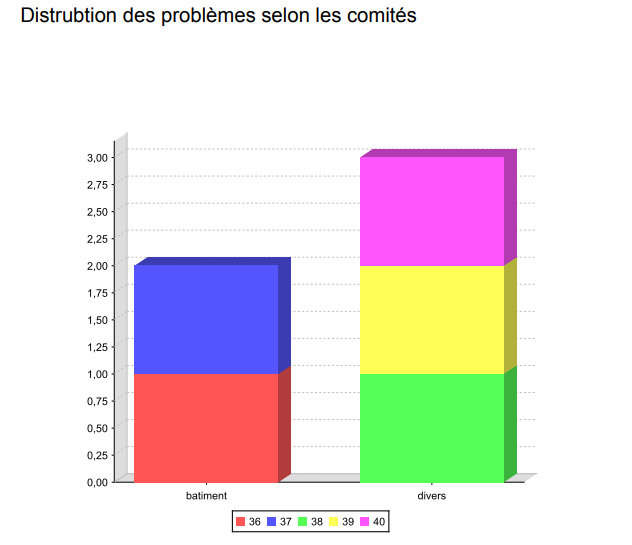
\includegraphics[width=500pt,height=400pt]{d2.png} 
		\caption{Distribution des problèmes selon les comités }
	\end{center}
	
\end{figure}
\newpage
\begin{figure}[h]
	
	\begin{center}
		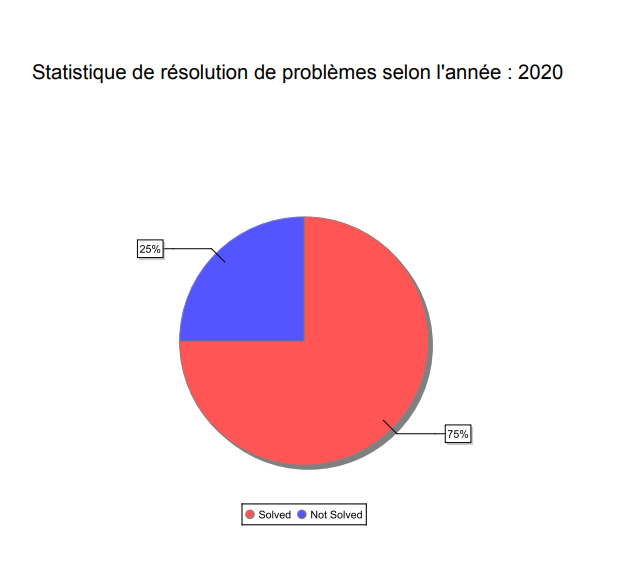
\includegraphics[width=500pt,height=400pt]{sg.png} 
		\caption{Statistiques globales}
	\end{center}
	
\end{figure}
\newpage
\begin{figure}[h]
	
	\begin{center}
		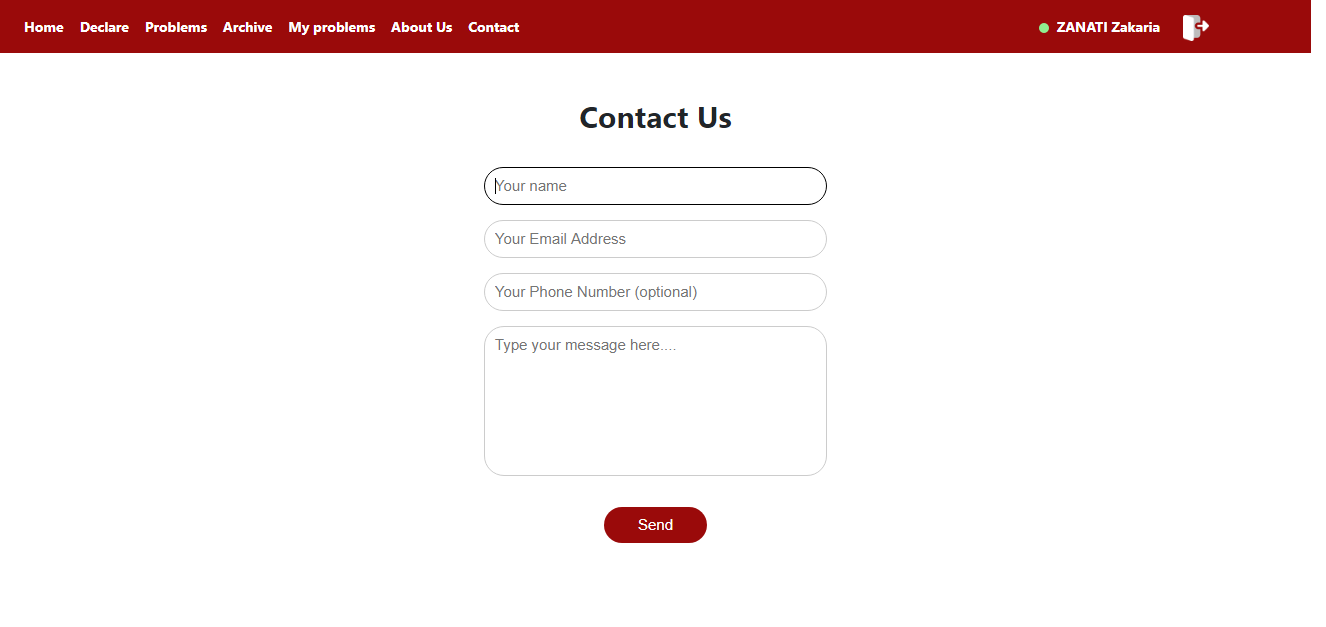
\includegraphics[width=500pt,height=300pt]{contactus.png} 
		\caption{Page contact us}
	\end{center}
	
\end{figure}
\newpage
\begin{figure}[h]
	
	\begin{center}
		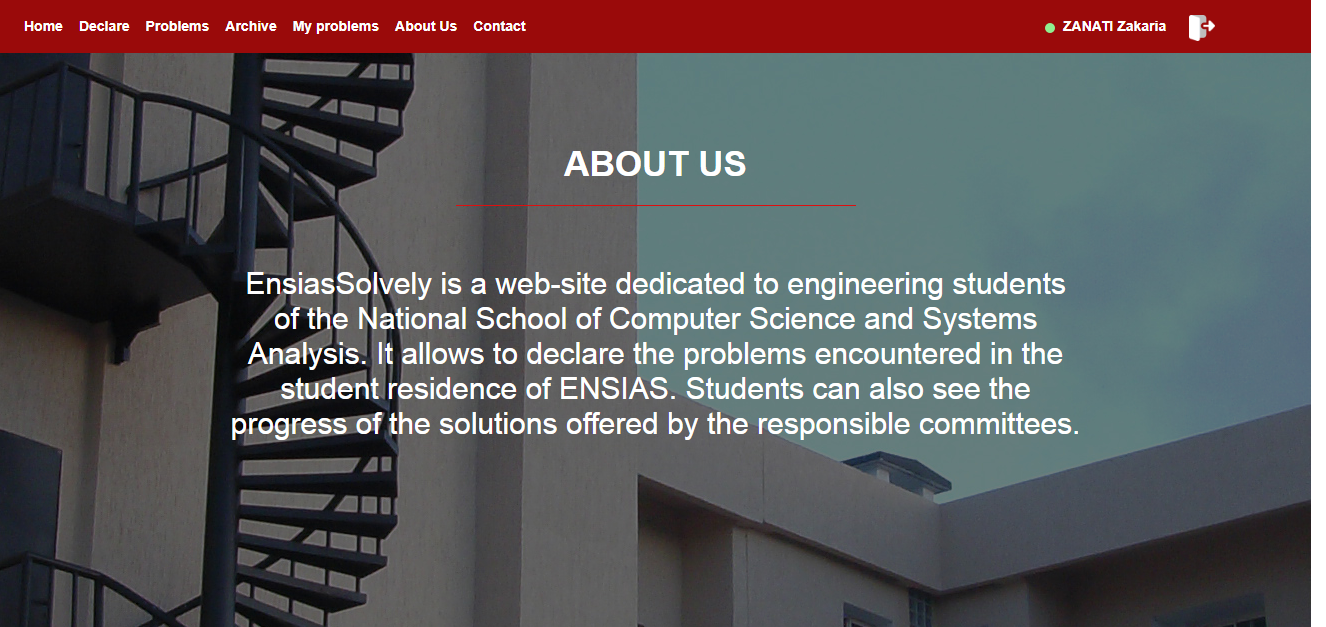
\includegraphics[width=500pt,height=350pt]{aboutus.png} 
		\caption{Page about us}
	\end{center}
	
\end{figure}
\newpage

\section{Conclusion}
Dans la première partie de ce chapitre, nous avons présenté l’environnement matériels et logiciels sur lesquels nous nous sommes basés pour réaliser ce travail. Puis nous avons  présenté les technologies utilisées. Par la suite, nous avons clôturé ce chapitre par une représentation des interfaces du site <Ensias Solvely> qui montrent les services offerts par notre application. S’il y’a un point qu’il fallait réussir tout de même c’est la partie «Comité» pour que le responsable puisse administrer le site Internet sans aucun problème.
	
\chapter*{Conclusion générale}
\addcontentsline{toc}{chapter}{Conclusion générale}	
Tout au long de ce rapport, nous avons présenté les différentes étapes de la réalisation de l’application du projet. Pour le développement de ce projet nous avons 
utilisé le langage UML, ce qui a permis de mener correctement la tâche d’analyse des besoins à l’aide du diagramme de cas d’utilisation et la tâche de conception, ainsi les scénarios sont aussi détaillés afin d’expliquer toutes les tâches faites puisque nous travaillons avec la technologie J2EE.

Ce projet nous a permis de développer nos compétences techniques, d’approfondir nos connaissances théoriques et pratiques, de stimuler un esprit d’initiative et de créativité, et notamment dans le domaine de développement des applications web. Il nous a donné la méthode pour assurer un travail de groupe, comment compter sur soi pour résoudre les problèmes au cas où ils se présentent, comment être professionnels dans notre travail, comment être attentifs aux indications de notre encadrant, comment être bien organisés pour accomplir dans les meilleurs délais, et meilleures conditions les tâches qui nous sont confiées. Ce projet nous a donné l’occasion de faire le lien entre les connaissances académiques, notamment en JAVA, Base de Données et le monde professionnel.

Notre application peut être aisément améliorée grâce à son aspect ouvert. Dans notre application, nous avons travaillé dans un réseau local. Pour la mettre en ligne nous avons seulement besoin de l’héberger sur un serveur.
\chapter*{Webographie}
\addcontentsline{toc}{chapter}{Webographie}	
[1]   https://openclassrooms.com/fr/courses/626954-creez-votre-application-web-avec-java-ee\\

[2]     https://docs.oracle.com/javaee/7/index.html\\

[3]    https://stackoverflow.com/ \\

[4]    https://www.supinfo.com/articles/single/3099-waterfall-model-modele-cascade \\

[5]   http://www.uml-sysml.org/documentation \\

[6]    https://www.w3schools.com/\\

[7]     https://www.supinfo.com/articles/single/2519-architecture-client-serveur \\  

\end{document}
